\documentclass[11pt]{report}

\usepackage{mathptmx}
\usepackage{url}
\usepackage{graphicx,pict2e,epic}
\usepackage{verbatim}

\newcommand*{\p}[1]{\textup{\texttt{#1}}}
\newcommand*{\ls}{\textsc{LearnSAT}}
\newcommand*{\pl}{\textsc{Prolog}}
\newcommand*{\sw}{\textsc{SWI-Prolog}}
\newcommand*{\dt}{\textsc{dot}}
\newcommand*{\ngg}{\mathop{\neg}}

\textwidth=15cm
\textheight=21cm
\topmargin=0pt
\headheight=0pt
\oddsidemargin=5mm
\headsep=0pt
\renewcommand{\baselinestretch}{1.1}
\setlength{\parskip}{0.20\baselineskip plus 1pt minus 1pt}
\parindent=0pt

\title{\bfseries \ls --- Tutorial\\\mbox{}\\\mbox{}\\
\bfseries\normalsize Version 1.5}

\author{\bfseries Mordechai (Moti) Ben-Ari\\\mbox{}\\
\url{http: //www.weizmann.ac.il/sci-tea/benari/}}

\begin{document}

\maketitle

\thispagestyle{empty}

\vspace*{\fill}

\begin{center}
\copyright{} 2012-13 by Mordechai (Moti) Ben-Ari.
\end{center}
This work is licensed under the Creative Commons Attribution-ShareAlike 3.0
License. To view a copy of this license, visit
\url{http://creativecommons.org/licenses/by-sa/3.0/}; or, (b) send a letter
to Creative Commons, 543 Howard Street, 5th Floor, San Francisco,
California, 94105, USA.

\vspace*{\fill}

\setcounter{page}{0}
\newpage

\chapter*{Overview}

\ls{} is a program for learning about SAT solving. It implements the
classic \emph{Davis-Putnam-Logemann-Loveland (DPLL)} algorithm, together
with modern extensions of the algorithm: \emph{conflict-driven clause
learning (CDCL)} and \emph{non-chronological backtracking (NCB)}.

For instructions on how to run \ls{} see the User's Guide in the \ls{}
distribution.

This document is a tutorial on SAT solving with \ls{}. The algorithms
and notation follow \cite{mlm}. Some printouts have been reformatted or
edited.

The tutorial assumes a basic knowledge of propositional logic such as
presented in Chapters~2 and~3 of \cite{mlcs}. The material is
summarized in Chapter~\ref{ch.intro} of the tutorial. For an
introduction to SAT solvers, see \cite[Chapter~6]{mlcs}. The
comprehensive reference is the \emph{Handbook of Satisfiability}
\cite{SAT}.

Chapter~\ref{ch.mlm} demonstrates \ls{} in great detail on the example
in \cite{mlm}. This is followed by several chapters using other examples
to demonstrate specific aspects of the algorithms.

\begin{center}
\framebox[.9\textwidth]{\parbox{.85\textwidth}{\ls{} can generate graphs in both color and
black-and-white. This document uses the black-and-white images for
printing. Color images of the same graphs can be found in the \ls{}
archive.}}
\end{center}

\chapter{Propositional logic}\label{ch.intro}

\begin{center}
\textbf{Definitions}
\end{center}

\begin{itemize}
\item There is an unbounded set $\mathcal{P}$, whose elements are called
\emph{propositional variables} or \emph{atoms}.
\item There is one unary operator \emph{negation}, denoted $\ngg$.
\item A \emph{literal} is an atom or the negation of an atom.
\item An atom is a \emph{positive literal} and the negation of an atom
is a \emph{negative literal}.
\item Let $l$ be a literal. $l^c$, the \emph{complement} of $l$, is $\ngg p$ if
$l=p$ for some atom p and is $p$ if $l=\ngg p$.
\item $\{l,l^c\}$ is a \emph{complementary pair of literals}.
\item A \emph{clause} is a set of literals.
\item The \emph{empty clause} is a clause that is the empty set.
\item A \emph{formula} (\emph{in clausal form}) is a set of clauses.
\item The \emph{empty formula} is a formula that is the empty set.

\item An \emph{interpretation} is a map $\mathcal{I}: \mathcal{P}
\rightarrow \{T,F\}$.

\item $\mathcal{I}(l)=T$, a literal $l$ is \emph{true} in an
interpretation, iff: $l$ is an atom $p$ and $\mathcal{I}(p)=T$, or $l$ is
the negation of an atom $p$ and $\mathcal{I}(p)=F$.
Otherwise, $\mathcal{I}(l)=F$, $l$ is \emph{false}.

\item $\mathcal{I}(C)=T$, a clause $C$ is \emph{true} in an
interpretation $\mathcal{I}$, iff: for \emph{at least one} $l\in C$,
$\mathcal{I}(l)=T$; otherwise ($\mathcal{I}(l)=F$ for \emph{all}
$l\in C$), $\mathcal{I}(C)=F$, $C$ is \emph{false}.

\item $\mathcal{I}(A)=T$, a formula $A$ is \emph{true} in an
interpretation, iff: for \emph{all} $C\in A$, $\mathcal{I}(C)=T$;
otherwise ($\mathcal{I}(C)=F$ for \emph{some} $C\in A$),
$\mathcal{I}(A)=F$, $A$ is \emph{false}.

\item A formula $A$ is \emph{satisfiable} if there exists an
interpretation $\mathcal{I}$ such that $\mathcal{I}(A)=T$; $\mathcal{I}$
\emph{satisfies} $A$. If there is no such interpretation, $A$ is
\emph{unsatisfiable}.

\item $\mathcal{I}$ is a \emph{partial interpretation} for $A$ if it
maps \emph{some} of the atoms in $A$ into $\{T,F\}$. A partial
interpretation $\mathcal{I}$ satisfies $A$ if any extension of
$\mathcal{I}$ satisfies $A$.

\item Let $A$ be a formula and let $\mathcal{I}$ be a partial
interpretation for $A$. $A'=\mathcal{I}(A)$, the formula obtained by
\emph{evaluating $A$ under $\mathcal{I}$}, is obtained by removing all
clauses $C\in A$ such that for some $l\in C$, $\mathcal{I}(l)=T$, and by
removing from the remaining clauses all literals $l'$ such
$\mathcal{I}(l')=F$.

\item (Syntactical) A clause $C$ is a \emph{unit clause} if $C$
has exactly one literal.

\item (Semantical) A clause $C$ is a \emph{unit clause} under a partial
interpretation $\mathcal{I}$ if for some $l'\in C$, $\mathcal{I}(l')=T$
and for all $l\in C, l\neq l'$, $\mathcal{I}(l)=F$.

\end{itemize}

\bigskip

\begin{center}
\textbf{Algorithms}
\end{center}

\textbf{Unit clause rule} Let $A$ be a formula, $C=\{l\}$ a unit clause
in $A$, and $\mathcal{I}$ a partial interpretation. Construct
$\mathcal{I}'$ as the partial interpretation obtained by adding
$\mathcal{I}(l)=T$. Construct $A'$ by evaluating $A$ under
$\mathcal{I}'(l)$ (delete $C$ and delete $l^{c}$ from every clause in
which it appears).

\textbf{Unit propagation} Repeat the unit clause rule obtaining $A',
A'', A''', \ldots$, and
$\mathcal{I}',\mathcal{I}'',\mathcal{I}''',\ldots$, until the unit
clause rule no longer applies.

\textbf{Resolution rule} Let $C_{1},C_{2}$ be clauses such that $l\in
C_{1},l^{c}\in C_{2}$. $C$, the \emph{resolvent} of $C_{1}$ and $C_{2}$,
is the clause $(C_{1}-\{l\}) \cup (C_{2}-\{l^{c}\})$. $C_{1}$ and
$C_{2}$ are the \emph{parent clauses} of $C$.

\bigskip

\begin{center}
\textbf{Theorems}
\end{center}

\begin{itemize}
\item Let $A'$ be obtained by the unit clause rule from a formula $A$
and a partial interpretation $\mathcal{I}$. $A'$ is satisfiable if and
only if $A$ is satisfiable. Therefore, the unit clause rule is sound.

\item Let $C$ be the resolvent of $C_1$ and $C_2$. $C$ is satisfiable if
and only if $C_1$ and $C_2$ are satisfiable under the same
interpretation. Therefore, the resolution rule is sound.

\item The empty clause is unsatisfiable. The empty formula is
satisfiable. Proof outline: Consider the unsatisfiable formula $p \wedge
\neg p$, which in clausal form is $\{\{p\}, \{\neg p\}\}$. Apply the
unit clause rule to $\{p\}$: delete the clause $\{p\}$ and delete the
literal $\neg p$ from the clause $\{\neg p\}$. The result is the formula
with the single empty clause $\{\{\}\}$, so the unit clause is
unsatisfiable. Now consider the satisfiable formula $p$, which in
clausal form is $\{\{p\}\}$. Apply the unit clause rule to obtain the
empty formula (empty set of clauses) $\{\}$. (Actually, the empty
formula is valid but we did not define validity.)

\end{itemize}

\newpage

\begin{center}
\textbf{Davis-Putnam-Logemann-Loveland (DPLL) algorithm}
\end{center}

\textbf{Input}: A formula $A$.\\
\textbf{Output}: Return \emph{unsatisfiable} or a (possibly partial)
interpretation that satisfies $A$.

The algorithm is expressed as the recursive function
$\textit{DPLL}(B,\mathcal{I})$ with parameters: a formula $B$ and a
partial interpretation $\mathcal{I}$. The initial call is
$\textit{DPLL}(A,\{\})$. 

\medskip

\noindent $\textit{DPLL}(B,\mathcal{I})$
\begin{itemize}

\item Perform unit propagation on $B$; let $B'$ and $\mathcal{I}'$ be
the final formula and partial interpretation.

\begin{itemize}
\item If $B'$ contains the empty clause, return \emph{unsatisfiable};
\item If $B'$ is the empty formula, return $\mathcal{I}'$;
\item (otherwise, continue).
\end{itemize}
\item \emph{Choose} an atom $p$ in $B'$, \emph{choose} a truth value
$\textit{val}$ as $T$ or $F$, and let $\mathcal{I}_1$ be the
partial interpretation obtained by adding the assignment
$p\rightarrow \textit{val}$  to $\mathcal{I}'$. 

\item \textit{result} $\leftarrow$ $\textit{DPLL}(B',\mathcal{I}_1)$.
\begin{itemize}
\item If \textit{result} is not \emph{unsatisfiable}, return \textit{result};
\item (otherwise, continue).
\end{itemize}

\item Let $\mathcal{I}_2$ be the partial interpretation obtained by
adding the assignment of $p\rightarrow \textit{val}^c$ to
$\mathcal{I}'$, where $\textit{val}^c = F$ if $\textit{val} = T$ and
$\textit{val}^c = T$ if $\textit{val} = F$.

\item \textit{result} $\leftarrow$ $\textit{DPLL}(B',\mathcal{I}_2)$.
\begin{itemize}
\item Return \textit{result}.
\end{itemize}
\end{itemize}



\chapter{A detailed example}\label{ch.mlm}

\section{The DPLL algorithm}

For the tutorial, we use the set of clauses from \cite{mlm} as our
example.\footnote{\ls{} tries decision assignments in lexicographic
order, so \p{x21} and \p{x31} had a \p{0} added to their names to
preserve the order in \cite{mlm}. From Version 1.3.1 of \ls{}, the order
can be specified, so this is no longer needed.}

\begin{verbatim}
  1. [x1,x031,~x2]   2. [x1,~x3]         3. [x2,x3,x4]
  4. [~x4,~x5]       5. [x021,~x4,~x6]   6. [x5,x6]
\end{verbatim}

The file \p{examples.pro} contains the predicate \p{mlm} that runs
\p{dpll} on this set of clauses:

\begin{verbatim}
mlm :-
  dpll( [  [x1, x031, ~x2], [x1, ~x3], [x2, x3, x4],
           [~x4, ~x5], [x021, ~x4, ~x6], [x5, x6]     ], _).
\end{verbatim}

When the DPLL algorithm is run on the set of clauses, it assigns
0 to \p{x021}, \p{x031} and \p{x1}:

\begin{verbatim}
?- mlm.
LearnSAT v1.4.0. Copyright 2012-13 by Moti Ben-Ari. GNU GPL.
Decision assignment: x021=0
Decision assignment: x031=0
Decision assignment: x1=0
\end{verbatim}

Clause 1 is now a unit clause \verb+[~x2]+ implying that \p{x2} must be
assigned 0; clause 2 is also a unit clause \verb+[~x3]+ implying that
\p{x3} must be assigned 0:

\begin{verbatim}
Propagate unit: ~x2 (x2=0) derived from: 1. [x1,x031,~x2]
Propagate unit: ~x3 (x3=0) derived from: 2. [x1,~x3]
\end{verbatim}

This in turn leads to a sequence of unit propagations until clause 6
is falsified:

\begin{verbatim}
Propagate unit:  x4 (x4=1) derived from: 3. [x2,x3,x4]
Propagate unit: ~x5 (x5=0) derived from: 4. [~x4,~x5]
Propagate unit: ~x6 (x6=0) derived from: 5. [x021,~x4,~x6]
Conflict clause: 6. [x5,x6]
\end{verbatim}

Now, the algorithm backtracks, trying the assignment of 1 to \p{x1} and
then 0 to \p{x2} and \p{x3}:
\begin{verbatim}
Decision assignment: x1=1
Decision assignment: x2=0
Decision assignment: x3=0
\end{verbatim}
which causes another sequence of unit propagations leading to the same
conflict clause:
\begin{verbatim}
Propagate unit:  x4 (x4=1) derived from: 3. [x2,x3,x4]
Propagate unit: ~x5 (x5=0) derived from: 4. [~x4,~x5]
Propagate unit: ~x6 (x6=0) derived from: 5. [x021,~x4,~x6]
Conflict clause: 6. [x5,x6]
\end{verbatim}

The algorithm backtracks to assign 1 to \p{x3}, followed by 0 to \p{x4}
and \p{x5}; then, unit propagation results in assigning 1 to \p{x6}:

\begin{verbatim}
Decision assignment: x3=1
Decision assignment: x4=0
Decision assignment: x5=0
Propagate unit: x6 derived from: 6. [x5,x6]
\end{verbatim}

The result is a set of assignments that satisfies the set of clauses:

\begin{verbatim}
Satisfying assignments:
[x021=0,x031=0,x1=1,x2=0,x3=1,x4=0,x5=0,x6=1]
Statistics: clauses=6, variables=8, units=9, decisions=9, conflicts=2
\end{verbatim}

\newpage

\section{Display options}

The trace of the algorithm shown in the previous section resulted from
the following display options that are selected by default:
\p{conflict}, \p{decision}, \p{result}, \p{sorted}, \p{unit}. The option
\p{sorted} displays the assignments as a sorted list; if the option is
cleared, the assignments will be displayed in the reverse order in which
they were made:

\begin{verbatim}
Satisfying assignments:
[x6=1,x5=0,x4=0,x3=1,x2=0,x1=1,x031=0,x021=0]
\end{verbatim}

Additional data may be obtained by using the following display options.

\begin{itemize}

\item Select \p{clause} to display the clauses and their position within
the set of clauses so that you don't have to refer back to the source
code:

\begin{verbatim}
Clauses to be checked for satisfiability:
1. [x1,x031,~x2],
2. [x1,~x3],
3. [x2,x3,x4],
4. [~x4,~x5],
5. [x021,~x4,~x6],
6. [x5,x6]
\end{verbatim}

\item Select \p{variable} to display the set of \emph{unassigned}
variables before each decision assignment and select \p{partial} to
display the set of assignments \emph{so far}:

\begin{verbatim}
Variables: [x021,x031,x1,x2,x3,x4,x5,x6]
Decision assignment: x021=0
Assignments so far:
[x021=0]
Variables: [x031,x1,x2,x3,x4,x5,x6]
Decision assignment: x031=0
Assignments so far:
[x031=0,x021=0]
Variables: [x1,x2,x3,x4,x5,x6]
Decision assignment: x1=0
Assignments so far:
[x1=0,x031=0,x021=0]
Propagate unit: ~x2 (x2=0) derived from: 1. [x1,x031,~x2]
Assignments so far:
[x2=0,x1=0,x031=0,x021=0]
\end{verbatim}

These options save the effort of frequent scrolling when tracing the
algorithm.

\item Select \p{assignment} to display the set of assignments that caused a
clause to become a conflict clause:
\begin{verbatim}
Conflict clause: 6. [x5,x6]
Conflict caused by assignments:
[x021=0,x031=0,x1=0,x2=0,x3=0,x4=1,x5=0,x6=0]
\end{verbatim}
This is an alternative to selecting \p{partial} because it just displays
the set of assignments when a conflict has been reached.

\item Select \p{evaluate} to display how each clause is evaluated when a
new assignment is tried:

\begin{verbatim}
Decision assignment: x021=0
Evaluate: [x021,~x4,~x6] has literal x021 deleted
Decision assignment: x031=0
Evaluate: [x1,x031,~x2] has literal x031 deleted
Evaluate: [x021,~x4,~x6] has literal x021 deleted
Decision assignment: x1=0
Evaluate: [x1,x031,~x2] has literal x1 deleted
Evaluate: [x1,x031,~x2] has literal x031 deleted
Evaluate: [x1,x031,~x2] is a unit clause
Evaluate: [x1,~x3] has literal x1 deleted
Evaluate: [x1,~x3] is a unit clause
Evaluate: [x021,~x4,~x6] has literal x021 deleted
Propagate unit: ~x2 (x2=0) derived from: 1. [x1,x031,~x2]
Evaluate: [x1,x031,~x2] has literal x1 deleted
Evaluate: [x1,x031,~x2] has literal x031 deleted
Evaluate: [x1,x031,~x2] is true
Evaluate: [x1,~x3] has literal x1 deleted
Evaluate: [x1,~x3] is a unit clause
\end{verbatim}
\textbf{Warning}: This display option results in extremely verbose output
and would only be used in the initial stages of learning about DPLL.

\end{itemize}

\newpage

\section{Assignment trees}

Select \p{tree} to see a tree of the assignments
(Figure~\ref{tree1}).\footnote{This tree is different from the standard
semantic tree where the nodes are the variables and the edges are the
assignments. Here, the nodes are the assignments and the edges are not
labeled.} The display option \p{label} was also selected to add the
antecedent clauses to nodes that implied by unit propagation.

\begin{figure}
\begin{center}
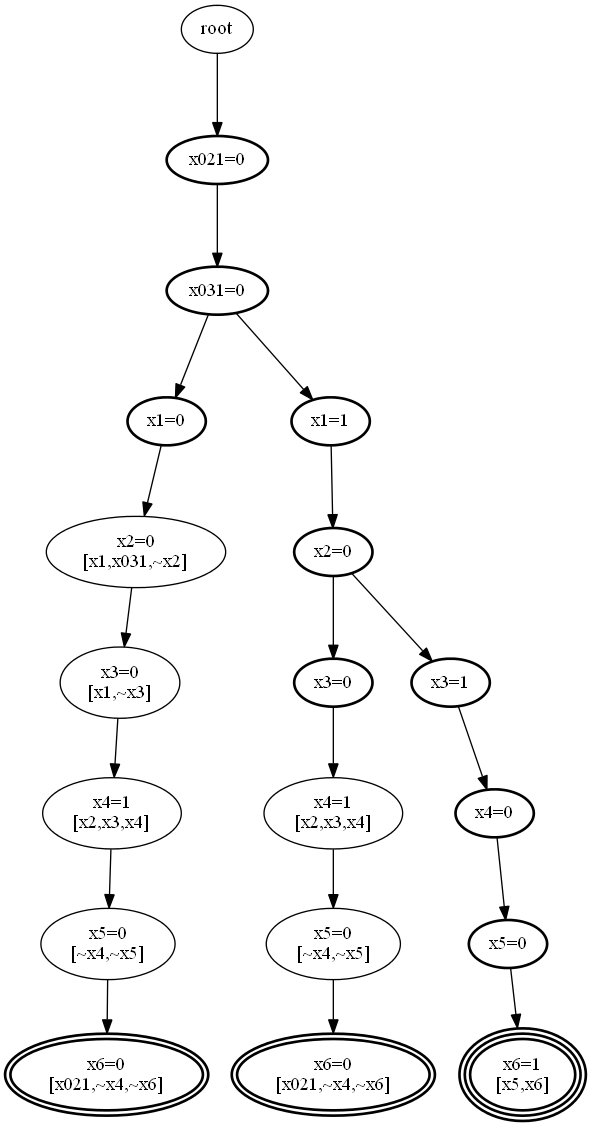
\includegraphics[keepaspectratio=true,height=.9\textheight]{tree1-bw}
\end{center}
\caption{Tree of assignments for the DPLL algorithm}\label{tree1}
\end{figure}

Decision assignments are in bold; assignments implied by unit
propagation are in black; conflict nodes have a double border; the node
where the satisfying assignments are found has a triple border. The
search backtracked to assign 1 to \p{x1} after trying 0 and to assign 1
to \p{x3} after trying 0.

Select \p{tree\_inc} to generate the trees incrementally, whenever a
conflict is reached.

\section{Improving efficiency with learned clauses}

Let us run the same example with conflict-directed clause learning by
setting the mode:

\begin{verbatim}
?- set_mode(cdcl).
\end{verbatim}

The display options relevant to this mode selected by default are:
\p{learned}, \p{resolvent}, \p{uip}.

After encountering the conflict clause \verb+[x5,x6]+, the algorithm
\emph{learns} the clause \verb+[x021,~x4]+ (Section~\ref{learned.res}).
When backtracking to assign 1 to \p{x3}, the learned clause becomes a
unit clause based upon the previous assignment of 0 to \p{x021}. Unit
propagation leads to a satisfying assignment:

\begin{verbatim}
Conflict clause: 6. [x5,x6]
  . . .
Learned clause from resolution (used): [x021,~x4]
Decision assignment: x1=1@3
Propagate unit: ~x4 (x4=0@3) derived from: 7. [x021,~x4]
Decision assignment: x2=0@4
Propagate unit:  x3 (x3=1@4) derived from: 3. [x2,x3,x4]
Decision assignment: x5=0@5
Propagate unit:  x6 (x6=1@5) derived from: 6. [x5,x6]
Satisfying assignments:
[x021=0@1,x031=0@2,x1=1@3,x2=0@4,x3=1@4,x4=0@3,x5=0@5,x6=1@5]
Statistics: clauses=6, variables=8, units=8, decisions=6, conflicts=1
\end{verbatim}
Assignments are displayed together with their levels. Each decision
assignment increases the level, while assignments implied by unit
propagation receive the level of the last decision assignment. 

The search with CDCL is more efficient: compare the statistics (6
decisions and 1 conflict instead of 9 decisions and 2 conflicts) or the
the tree of assignments (Figure~\ref{tree2}).

\begin{figure}
\begin{center}
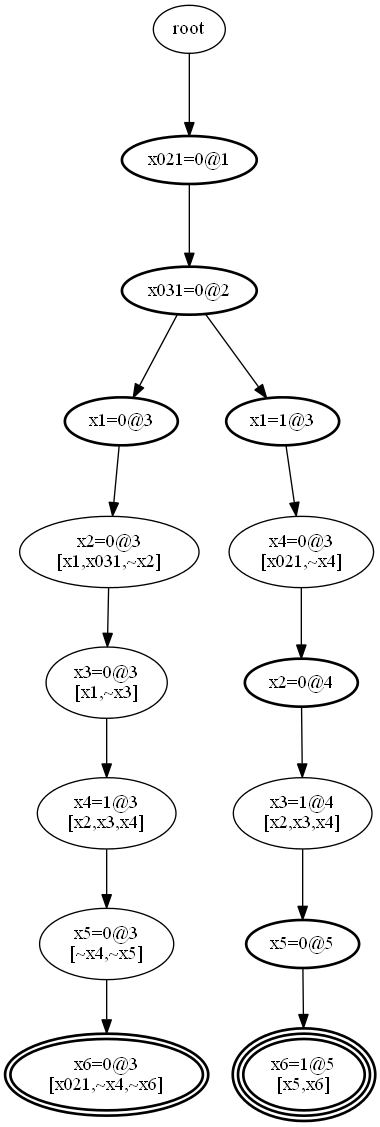
\includegraphics[keepaspectratio=true,height=.9\textheight]{tree2-bw}
\end{center}
\caption{Tree of assignments for the DPLL algorithm with CDCL}\label{tree2}
\end{figure}

\clearpage

\section{The implication graph}

When a conflict clause is found, an \emph{implication graph} is
constructed and used to learn a clause. Select \p{graph} to display a
textual representation of a graph: a list of nodes and a list of
edges labeled with the antecedent clauses (because \p{label} was also
selected):

\begin{verbatim}
Implication graph:
[kappa, x021=0@1, x031=0@2, x1=0@3, x2=0@3, x3=0@3, x4=1@3, x5=0@3, x6=0@3]
[
x021=0@1 --5.[x021,~x4,~x6]--> x6=0@3,
x031=0@2 --1.[x1,x031,~x2]--> x2=0@3,
x1=0@3 --1.[x1,x031,~x2]--> x2=0@3,
x1=0@3 --2.[x1,~x3]--> x3=0@3,
x2=0@3 --3.[x2,x3,x4]--> x4=1@3,
x3=0@3 --3.[x2,x3,x4]--> x4=1@3,
x4=1@3 --4.[~x4,~x5]--> x5=0@3,
x4=1@3 --5.[x021,~x4,~x6]--> x6=0@3,
x5=0@3 --6.[x5,x6]--> kappa,
x6=0@3 --6.[x5,x6]--> kappa
]
\end{verbatim}

Select \p{dot} to generate a \dt{} representation of the
graph:

\begin{center}
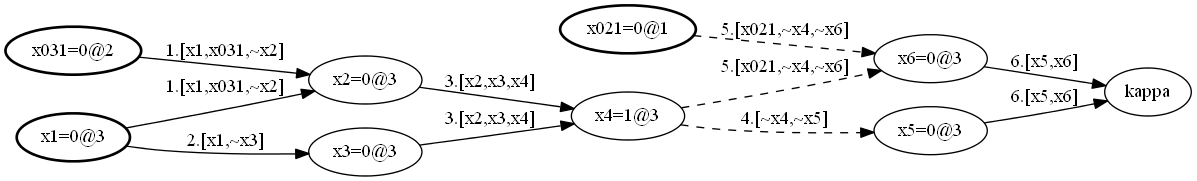
\includegraphics[keepaspectratio=true,width=\textwidth]{graph-bw}
\end{center}

Options \p{incremental} and \p{dot\_inc} generate the graphs after each
step of the algorithm, not just when a conflict clause is reached.

The implication graph represents the result of unit propagation that
leads to a conflict, starting from a set of decision assignments. In the
graph, are three source nodes, one for each of the decision assignments
(\p{x021=0@1}, \p{x031=0@2}, \p{x1=0@3}) that together lead to a
conflict by unit propagation.

The conflict is represented by the sink node \p{kappa} and the
assignments implied by unit propagation are represented by nodes labeled
with the assignments. An edge of the graph is labeled with the
\emph{antecedent} clause of its target node. This is the unit clause
that implied the assignment labeling that node. For example, the
decision assignments \p{x1=0@3}, \p{x031=0@2} cause \verb+[x1,x031,~x2]+
to become a unit clause \verb+[~x2]+ and therefore this clause implies
the assignment of 0 to \p{x2}. The assignment receives the same level as
the last decision assignment so its node is labeled \p{x2=0@3}.

For each non-source node, there is an incoming edge for each literal in
the unit clause except the one whose assignment is being implied. The
source nodes of these edges are the ones labeled with the assignments to
those literals. Since the clause \verb+[x1,x031,~x2]+ with three
literals implied the assignment \p{x2=0@3}, the node labeled \p{x2=0@3}
has two incoming edges: one from the node \p{x1=0@3} that assigned 0 to
\p{x1} and one from the node \p{x031@2} that assigned 0 to \p{x031}.

The implication graph shows that the decision assignments \p{x021=0@1},
\p{x031=0@2}, \p{x1=0@3} cause a conflict. Clearly, if
\verb+[x021,x031,x1]+ were a clause in the original set of clauses, it
would be evaluated when the decisions were made. Since it evaluates to
0, it is a conflict clause that would be found immediately and there
would be no need to carry out unit propagation. Therefore, by
\emph{learning} this clause---adding it to our original set of
clauses---any subsequent decision assignments that include these three
would \emph{immediately} lead to the discovery of a conflict.

Unfortunately, there is no advantage to learning a clause based only on
these decision assignments, because the same set of decisions at levels
1, 2 and 3 will never occur again after backtracking.

Sections~\ref{learned.dom}--\ref{learned.res} present algorithms that
can find \emph{shorter} learned clauses that are more likely to become
conflict clauses as the algorithm continues. Section~\ref{learned.dom}
describes how to learn a clause by computing a dominator in the
implication graph and Section~\ref{learned.res} describes how to learn a
clause resolving backwards from the conflict node.

The two algorithms are always run one after the other, but only the
clause learned by resolution is actually learned. You can trace either
or both of the algorithms. Display option \p{dominator} traces the
computation of a dominator, and the options \p{learned}, \p{resolvent}
and \p{uip} trace the computation by resolution.

\newpage

\section{Learning a clause from a dominator}\label{learned.dom}

Here again is the implication graph:

\begin{center}
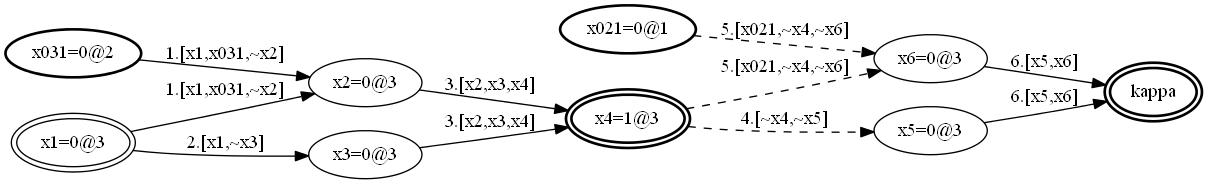
\includegraphics[keepaspectratio=true,width=\textwidth]{dom-bw}
\end{center}

Consider all the (four) paths from the \emph{last} decision assignment
(\p{x1=0@3} with a double border) to the node labeled \p{kappa} (also
with a double border). A node (\p{x4=1@3} with a double border) is
called a \emph{dominator} of a decision node if it appears on all the
paths from the decision node to \p{kappa}. \ls{} computes the paths and
finds a dominator:

\begin{verbatim}
Paths from the decision node at this level to kappa:
x1=0@3 --> x2=0@3 --> x4=1@3 --> x5=0@3 --> kappa
x1=0@3 --> x2=0@3 --> x4=1@3 --> x6=0@3 --> kappa
x1=0@3 --> x3=0@3 --> x4=1@3 --> x5=0@3 --> kappa
x1=0@3 --> x3=0@3 --> x4=1@3 --> x6=0@3 --> kappa
A dominator is: x4=1@3
\end{verbatim}

A dominator is a \emph{unique implication point (UIP)} because its
assignment participates in the conflict in the same way as do \emph{all}
the decision assignments that it dominates. Here, the assignment
\p{x4=1@3} is implied by the \emph{two} assignments \p{x031=0@2} and
\p{x1=0@3}, so \verb+~x4+ can replace \p{x031} and \p{x1} in the learned
clause \verb+[x021,x031,x1]+ to obtain a shorter learned clause
\verb+[x021,~x4]+.

There remains one path from a decision node to \p{kappa} that does not
contain the dominator:
\begin{verbatim}
Paths from decision nodes at lower levels to kappa:
x021=0@1 --> x6=0@3 --> kappa
\end{verbatim}

The learned clause is therefore composed of the complement of the
assignment at the UIP, together with the complements of assignments at
\emph{lower} levels that are not dominated by the UIP. The literal
chosen for this path is the one just before the path joins an assignment
at the highest level; in this case, it is the decision assignment to
\verb+x021+:

\begin{verbatim}
Learned clause from dominator (not used): [x021,~x4]
\end{verbatim}

The dotted lines form a \emph{cut}: their source nodes are the
assignments that define the literals in the learned clause. These nodes
define a learned clause because assignments to the literals necessarily
lead to the conflict. The cut we chose includes the edges whose source
node is the UIP together with an edge on each path from a decision node
that is not dominated by the UIP.

\newpage

\section{Learning a clause by resolution}\label{learned.res}

The learned clause can be obtained by resolution starting with the
conflict clause---the antecedent clause of the \p{kappa} node---and
terminating when a UIP is found. Define the conflict clause as the
initial \emph{current clause}. At each step, the antecedent clause at
the current node clashes with the current clause on the literal that was
assigned at that node by unit propagation. For example, given the
initial current clause \verb+[x5,x6]+, \p{x5} was assigned by unit
propagation at this level, so we can resolve \verb+[x5,x6]+ with the
antecedent clause \verb+[~x4,~x5]+ to obtain the resolvent
\verb+[~x4,x6]+ which becomes the current clause. The next step is to
resolve this clause with \verb+[x021,~x4,~x6]+, the antecedent of the
assignment to \p{x6}, to obtain \verb+[x021,~x4]+. The resolution now
terminates because clause is associated with a UIP: there is one
(implied) literal assigned at the current level and the other literals
were assigned by decision assignments at lower levels.

\begin{verbatim}
Conflict clause: 6. [x5,x6]
Not a UIP: two literals [x6,x5] are assigned at level: 3
Resolvent: of [x5,x6] and antecedent [x021,~x4,~x6] is [x5,x021,~x4]
Not a UIP: two literals [~x4,x5] are assigned at level: 3
Resolvent: of [x5,x021,~x4] and antecedent [~x4,~x5] is [x021,~x4]
UIP: one literal ~x4 is assigned at level: 3
Learned clause from resolution (used): [x021,~x4]
\end{verbatim}

Since the conflict clause is unsatisfiable under the current set of
decision assignments, so is the set consisting of it and its clashing
clause, and therefore their resolvent---the next current clause---is
also unsatisfiable.

For example, \verb+[x5,x6]+ is a conflict clause because it evaluates to
0. The antecedent clause \verb+[~x4,~x5]+ is a unit clause and therefore
exactly one literal is assigned 1. Since both literals in the conflict
clause \verb+[x5,x6]+, are assigned 0, \verb+~x5+, the complement of
\verb+x5+, is assigned 1, so it must be the \emph{only} literal in the
antecedent clause \verb+[~x4,~x5]+ that is assigned 1. Therefore,
\verb+~x4+ is assigned 0 and we conclude that all literals in the
resolvent \verb+[~x4,x6]+ are assigned 0.

Which of these clauses should we learn? Successive resolution steps will
eventually lead back to the clause defined by the decision nodes
(\verb+[x021,x031,x1]+), but there is no advantage to learning this
clause. However, the resolvent clause associated with a UIP
(\verb+[x021,~x4]+) contains only a single literal at the current level
(\verb+~x4+), so it can replace the decision literal at the same level
(\verb+x1+), as well as any decision variables at lower levels that are
dominated by the UIP (\verb+x031+).


\clearpage

\section{Non-chronological backtracking}

Let us now select the NCB mode:
\begin{verbatim}
?- set_mode(ncb).
\end{verbatim}

When a learned clause has been obtained, the backtrack level for
non-chronological backtracking is computed. This is the highest level of
an assignment in the learned clause except for the current level. In the
example, the learned clause is \verb+[x021,~x4]+, where \p{x4} was
assigned at level 3, the current level, and \p{x021} was assigned at
level 1, which becomes the backtrack level. When backtracking, we can
skip decision assignments whose level is at a lower level than the
backtrack level, in the example, the decision assignments at levels 3
and 2:

\begin{verbatim}
Non-chronological backtracking to level: 1
Skip decision assignment: x1=1@3
Skip decision assignment: x031=1@2
\end{verbatim}

Once 0 is assigned to \p{x021}, the clause \verb+[x021,~x4]+ becomes a
unit clause \verb+[~x4]+ which forces the assignment of 1 to \p{x4}. But
we already know (cf. the implication graph) that those two assignments
are sufficient to cause a conflict. It follows that there is no point in
exploring the other assignments to \p{x031} and \p{x1}: \emph{the
assignments to \p{x021} and \p{x4} are sufficient by themselves to cause
a conflict}.

NCB can be seen in the tree of assignments (Figure~\ref{tree3}). The
graph is no longer a tree but a DAG (directed acyclic graph) because
once \p{x021} is assigned (0 or 1), the assignments of 0 to \p{x031} and
then \p{x1} lead to the same sequence of unit propagations. The graph
branches only at its leaves because one assignment leads to a conflict
clause and the other to a satisfying assignment.

\begin{figure}
\begin{center}
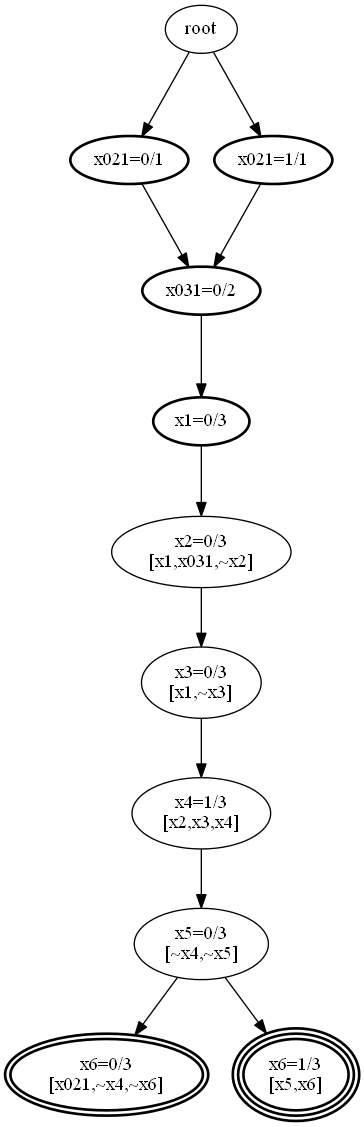
\includegraphics[keepaspectratio=true,height=.9\textheight]{tree3-bw}
\end{center}
\caption{Tree of assignments for the DPLL algorithm with CDCL and NCB}\label{tree3}
\end{figure}

\clearpage

\chapter{The pigeonhole principle}\label{ch.pigeon}

The pigeonhole principle states that if we place $n+1$ pigeons in $n$
holes then one hole contains at least two pigeons. Therefore, a formula
stating that all pigeons are in different holes must be unsatisfiable.
Let \p{pij} be an atom whose intended meaning is that pigeon \p{i} is in
hole \p{j}; for two holes and three pigeons, the set of clauses is:

\begin{verbatim}
  [p11, p12],   [p21, p22],   [p31, p32],   % Each pigeon in hole 1 or 2 
  [~p11, ~p21], [~p11, ~p31], [~p21, ~p31], % No pair is in hole 1
  [~p12, ~p22], [~p12, ~p32], [~p22, ~p32], % No pair is in hole 2
\end{verbatim}

and for three holes and four pigeons the formula is:

\begin{verbatim}
  % Each pigeon in at least hole
  [p11, p12, p13], [p21, p22, p23], [p31, p32, p33], [p41, p42, p43], 
  % Each hole has at most one pigeon
  [~p11, ~p21], [~p11, ~p31], [~p11, ~p41],
  [~p21, ~p31], [~p21, ~p41], [~p31, ~p41],
  [~p12, ~p22], [~p12, ~p32], [~p12, ~p42],
  [~p22, ~p32], [~p22, ~p42], [~p32, ~p42],
  [~p13, ~p23], [~p13, ~p33], [~p13, ~p43],
  [~p23, ~p33], [~p23, ~p43], [~p33, ~p43]
\end{verbatim}

For the two-hole formula, the mode chosen makes no difference, but for
the three-hole formula, NCB makes a significant improvement:

\begin{verbatim}
dpll: units=49, decisions=16, conflicts=9
cdcl: units=42, decisions=16, conflicts=9
ncb:  units=25, decisions=10, conflicts=3
\end{verbatim}

If you look at the trace in NCB mode, the following clauses are
learned:

\begin{verbatim}
[p43,p33,~p22],   [p42,p32,~p23],  [p41,p31,~p23]
\end{verbatim}

Six decision assignments are skipped---both 0 and 1 for the variables
\p{p12}, \p{p13} and \p{p22}---so there are only three conflict instead
of nine.

Let us look now at the implication graphs. The graph for the two-hole
formula is shown in Figure~\ref{pigeon2} (shown top-to-bottom instead of
left-to-right). The conflict clause is \verb+[~p12,~p32]+ (stating
that either pigeon~1 or pigeon~3 is not in hole 2) and the
dominator is the node labeled \verb+p12=1@1+. Since \emph{all} nodes
are assigned at level~1, by resolving backwards we should be able to
learn the (unit) clause \verb+[~p12]+.

\begin{figure}
\begin{center}
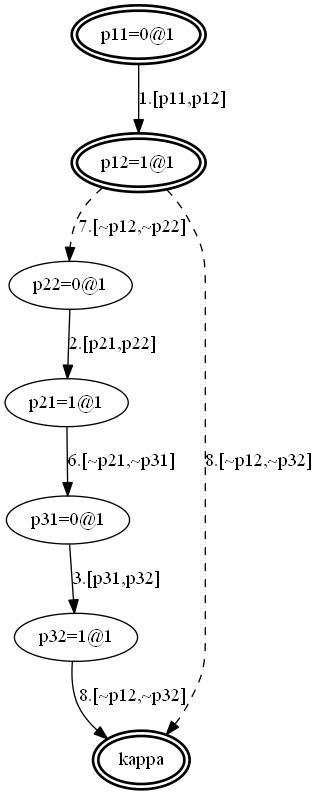
\includegraphics[keepaspectratio=true,height=.9\textheight]{pigeon2-bw}
\end{center}
\caption{Implication graph for two-hole pigeonhole}\label{pigeon2}
\end{figure}

However, we must be careful. According to \cite[p.~137]{mlm}: ``at each
step $i$, a literal $l$ assigned at the current decision level $d$ is
selected and the intermediate clause (\ldots) is resolved with the
antecedent of $l$.'' If we \emph{select} \verb+~p12+ and resolve it with
\verb+[p11,p12]+, the antecedent of the second node from the top, the
result is \verb+[p11,~p32]+, which is actually worse than just taking
the decision node \verb+[p11]+. When selecting the literal to resolve,
we must be careful to choose the \emph{last} one that was assigned, here
\verb+~p32+. If this is done, the sequence of resolvents is:

\begin{verbatim}
Conflict clause: 8. [~p12,~p32]
Resolvent: of [~p12,~p32] and antecedent [p31,p32] is [~p12,p31]
Resolvent: of [~p12,p31] and antecedent [~p21,~p31] is [~p12,~p21]
Resolvent: of [~p12,~p21] and antecedent [p21,p22] is [~p12,p22]
Resolvent: of [~p12,p22] and antecedent [~p12,~p22] is [~p12]
UIP: one literal ~p12 is assigned at level: 1
Learned clause from resolution: [~p12]
\end{verbatim}

The implication graph for the three-hole formula is shown in
Figure~\ref{pigeon3}. The node labeled \verb+p22=1@3+ is a dominator and
the clause learned by resolution is \verb+[p43,p33,~p22]+. The dashed
line shows the \emph{cut}: it is sufficient to assign to the three
literals before the cut in order to obtain a conflict, and the
complements of these literals form the learned clause.

The literals that form part of the learned clause come from assignments
at lower levels that are \emph{not} decision assignments, but
assignments implied by unit propagation: \verb+p43+ and \verb+p33+ which
are assigned at level~2.

\begin{figure}
\begin{center}
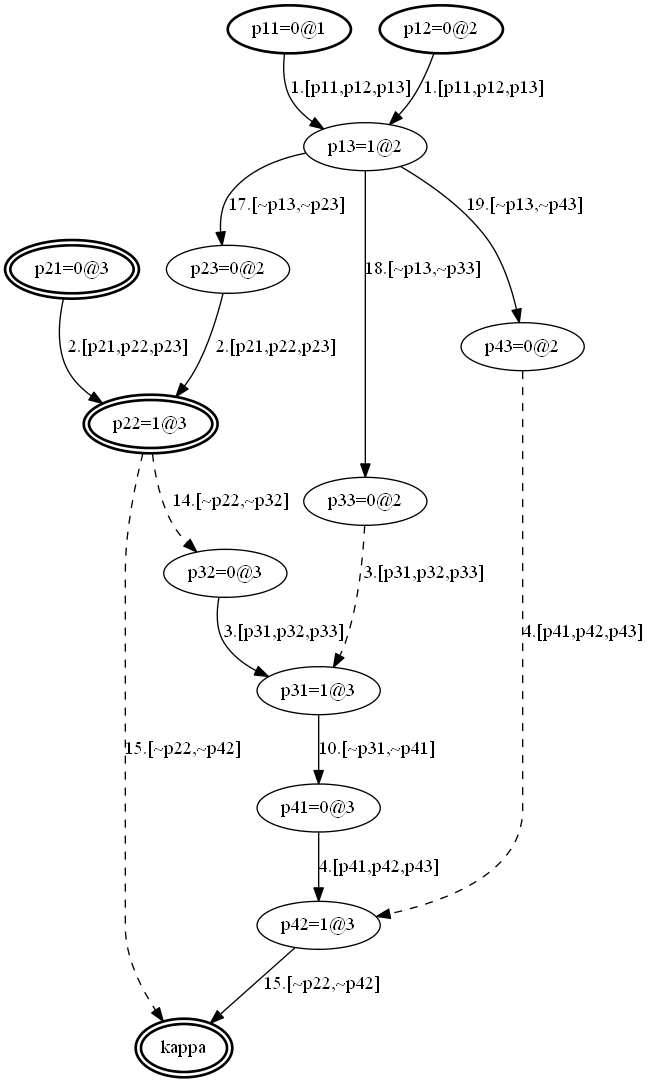
\includegraphics[keepaspectratio=true,height=.9\textheight]{pigeon3-bw}
\end{center}
\caption{Implication graph for three-hole pigeonhole}\label{pigeon3}
\end{figure}

\clearpage

\chapter{The four-queens problem}\label{ch.queens}

The $n$-queens problem is to place $n$ queens on an $n \times n$ chess
board such that no queen can capture another. It is usually posed in the
context of an standard $8\times 8$ board, but for simplicity we look at
a $4\times 4$ board. A solution is:

\begin{center}
\unitlength=1.0pt
\begin{picture}(100,100)
\put(0,0){
  \multiputlist(20,0)(20,0){1,2,3,4}
  \multiputlist(0,20)(0,20){4,3,2,1}
}
\put(10,10){
  \put(0,0){\grid(80,80)(20,20)}
  \put( 0, 20){\makebox(20,20){Q}}
  \put(20, 60){\makebox(20,20){Q}}
  \put(40,  0){\makebox(20,20){Q}}
  \put(60, 40){\makebox(20,20){Q}}
}
\end{picture}
\end{center}

The problem can be encoded in clausal form using 80 clauses on 16
variables \cite[Section~6.4]{mlcs}. Other encodings are discussed in
\cite[Section 2.3.1]{cnf} based on \cite{nadel}. The 4-queens problem
has a solution (in fact, two solutions), so the formula will be
satisfiable and the satisfying assignments provide a solution:

\begin{verbatim}
[p11=0,p12=0,p13=1,p14=0,p21=1,p22=0,p23=0,p24=0,
 p31=0,p32=0,p33=0,p34=1,p41=0,p42=1,p43=0,p44=0]
\end{verbatim}
where \p{pij} is true if a queen is placed in column \p{i} and row \p{j}. 

The statistics for the different modes are:
\begin{verbatim}
dpll: units=30, decisions=6, conflicts=2
cdcd: units=30, decisions=6, conflicts=2
ncb:  units=25, decisions=5, conflicts=1
\end{verbatim}

\newpage

If you examine the assignment tree for the DPLL algorithm (not shown),
you will see the effectiveness of unit propagation. Just three decision
assignments (\p{p11=0@1}, \p{p12=0@2}, \p{p13=0@3}) imply the assignment
\p{p14=1@3}, which in turn implies more assignments of 0 along its row and
diagonal. The placement of the first queen is shown on the left of
Figure~\ref{queens}, where the subscripts denote the assignment level and
primes denote the inferred assignments.

\begin{figure}[tb]
\begin{center}
\begin{tabular}{l@{\hspace{.2\textwidth}}r}
\unitlength=1.0pt
\begin{picture}(100,100)
\put(0,0){
  \multiputlist(20,0)(20,0){1,2,3,4}
  \multiputlist(0,20)(0,20){4,3,2,1}
}
\put(10,10){
  \put(0,0){\grid(80,80)(20,20)}
  \put( 0, 20){\makebox(20,20){$0_3$}}
  \put( 0, 40){\makebox(20,20){$0_2$}}
  \put( 0, 60){\makebox(20,20){$0_1$}}
  \put( 0, 0){\makebox(20,20){$1'_3$}}
  \put(20, 0){\makebox(20,20){$0'_3$}}
  \put(40, 0){\makebox(20,20){$0'_3$}}
  \put(60, 0){\makebox(20,20){$0'_3$}}
  \put(20,20){\makebox(20,20){$0'_3$}}
  \put(40,40){\makebox(20,20){$0'_3$}}
  \put(60,60){\makebox(20,20){$0'_3$}}
}
\end{picture}
&
\begin{picture}(100,100)
\put(0,0){
  \multiputlist(20,0)(20,0){1,2,3,4}
  \multiputlist(0,20)(0,20){4,3,2,1}
}
\put(10,10){
  \put(0,0){\grid(80,80)(20,20)}
  \put( 0, 20){\makebox(20,20){$0_3$}}
  \put( 0, 40){\makebox(20,20){$0_2$}}
  \put( 0, 60){\makebox(20,20){$0_1$}}
  \put( 0, 0){\makebox(20,20){$1'_3$}}
  \put(20, 0){\makebox(20,20){$0'_3$}}
  \put(40, 0){\makebox(20,20){$0'_3$}}
  \put(60, 0){\makebox(20,20){$0'_3$}}
  \put(20,20){\makebox(20,20){$0'_3$}}
  \put(40,40){\makebox(20,20){$0'_3$}}
  \put(60,60){\makebox(20,20){$0'_3$}}
  \put(20,60){\makebox(20,20){$0_4$}}
  \put(20,40){\makebox(20,20){$1'_4$}}
  \put(60,40){\makebox(20,20){$0'_4$}}
  \put(60,20){\makebox(20,20){$1'_4$}}
  \put(40,20){\makebox(20,20){$0'_4$}}
  \put(40,60){\makebox(20,20){$1'_4$}}
}
\end{picture}
\end{tabular}
\caption{Decisions and implications for the four-queens
problem}\label{queens}
\end{center}
\end{figure}

The next decision assignment is \p{p21=0@4} or \p{p21=1@4}, both of
which lead to conflicts. Let us look at \p{p21=0@4}. \p{p21=0@4} implies
\p{p22=1@4} because there has to be a queen in the second column. The
next implications are \p{p42=0@4}, \p{p43=1@4}, \p{p33=0@4}, \p{p31=1@4}
(see the right of Figure~\ref{queens}). Clearly, there is a conflict
because the clause \verb+[~p22,~p31]+ is false. The intended meaning of
this clause is that either there is no queen in (column 2, row 2) or
there is no queen in (column 3, row 1) because they can capture each
other.

We leave it to the reader to examine the sequence of assignments
following the decision assignment \p{p21=1@4} and to show that it too
leads to a conflict.

Figure~\ref{queens-ig} shows the implication graph with the dominator
node \verb+p22=1@4+ and the cut that defines the learned clause
\verb+[~p22,p32,p34,p41,p44]+. The learned clause is such that the
decision assignments at the lower levels (\verb+p11=0@1+,
\verb+p12=0@2+, \verb+p13=0@3+) make it a unit clause \verb+[~p22]+ and
force the assignment \p{p22=1@4}, regardless of the assignment to
\p{p21}. Therefore, non-chronological backtracking can skip the
assignment \p{p21=1@4} and continue with the previous decision
assignment. The assignment \p{p13=1@3} instead of \p{p13=0@3} leads to a
satisfying assignment by unit propagation alone!
 
\begin{figure}[b]
\begin{center}
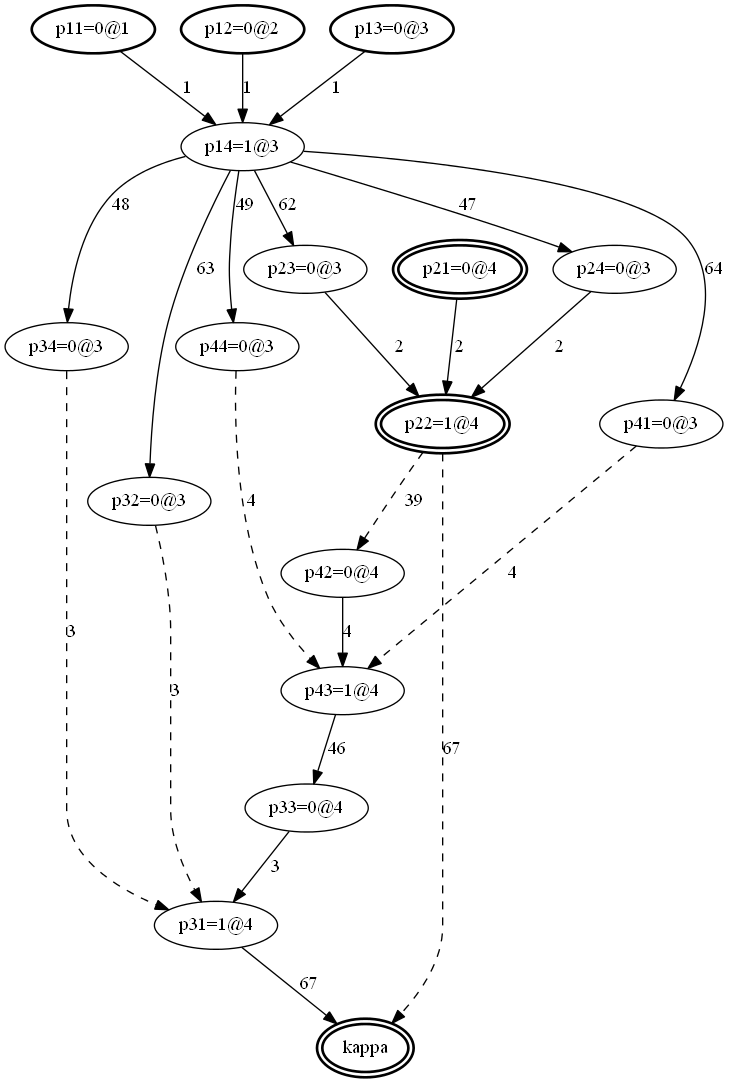
\includegraphics[keepaspectratio=true,height=.9\textheight]{queens-bw}
\end{center}
\caption{Implication graph for the four-queens}\label{queens-ig}
\end{figure}


\chapter{Tseitin graph formulas}\label{ch.tseitin}

G.S. Tseitin used formulas associated with graphs in his research on the
complexity of resolution.\footnote{See \cite[Section 4.5]{mlcs} for a
formal presentation of Tseitin formulas.} Consider the following
connected undirected graph whose vertices are labeled with 0 or 1 and
whose edges are labeled with letters:

\begin{center}
\unitlength=1.0pt
\begin{picture}(100,100)
\put(10,10){\framebox(80,80){\ }}
\put(10,10){\line(1,1){80}}
\put(0,0){\makebox(10,10){$0$}}
\put(45,0){\makebox(10,10)[b]{$t$}}
\put(90,0){\makebox(10,10){$0$}}
\put(0,45){\makebox(10,10)[l]{$q$}}
\put(40,45){\makebox(10,10)[l]{$r$}}
\put(90,45){\makebox(10,10)[r]{$s$}}
\put(0,90){\makebox(10,10){$0$}}
\put(45,90){\makebox(10,10)[t]{$p$}}
\put(90,90){\makebox(10,10){$1$}}
\end{picture}
\end{center}

The formula associated with this graph is defined as follows: for
each vertex, construct the set of clauses whose atoms are the letters
labeling the incident edges, such that the parity (sum modulo 2) of the
number of negated literals is not equal to the label of the vertex:

\begin{verbatim}
[~p, q], [p, ~q],
[p, r, s], [~p, ~r, s], [~p, r, ~s], [p, ~r, ~s],
[~s, t], [s, ~t],
[~q, r, t], [q, ~r, t], [q, r, ~t], [~q, ~r, ~t]
\end{verbatim}

For example, since $\{p, r, s\}$ are incident with a vertex labeled 1,
the number of negated literals in a cluase on these atoms has to be 0 or
2.

If the number of vertices labeled 1 is odd, the formula is
unsatisfiable.

\newpage

Let us look at the implication graph:

\begin{center}
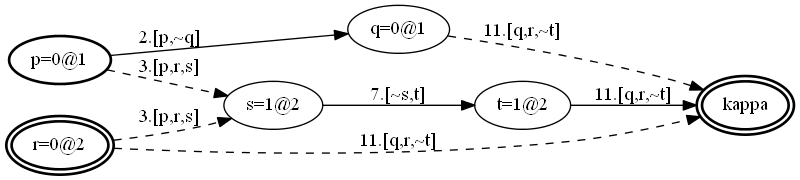
\includegraphics[keepaspectratio=true,width=\textwidth]{tseitin-ex-bw}
\end{center}

The only dominator of the highest-level decision node \verb+r=0@2+ is
the decision node itself. Since it is not implied by other decision
node, we cannot skip it in backtracking and the assignment \verb+r=1@2+
will have to be tried.

Another anomaly of this example is that the clause that would be learned
from the dominator is not the same as the one learned by resolution. The
former is \verb+[p,r]+, which is the complement of the dominator
decision node \verb+r=0@2+ and the decision node at a lower level
\verb+p=0@1+. The clause learned by resolution is obtained as follows:

\begin{verbatim}
Conflict clause: 11. [q,r,~t]
Resolvent: of [q,r,~t] and antecedent [~s,t] is [q,r,~s]
Resolvent: of [q,r,~s] and antecedent [p,r,s] is [q,p,r]
UIP: one literal r is assigned at level: 2
Learned clause from resolution: [q,p,r]
\end{verbatim}

This is a weaker clause than that defined by the dominator.

\chapter{Bounded model checking}\label{ch.model}

\section{Overview of model checking}

Model checking a method for verifying the correctness of computer
hardware and software. A model checker inputs a formal description of a
system and a correctness claim and then searches for states in the
execution of the system that falsify the claim.

In \emph{explicit-state} model checkers, the reachable states of the
system are generated one-by-one and the correctness claim is evaluated
after each new state is evaluated. If the system has a finite number of
states (and it is usually possible to construct a finite system by
abstracting away detail), eventually the model checker will either find
a state falsifying the claim or declare that the claim is true in all
reachable states. Clever algorithms and optimized data structures ensure
that many real systems can be completely checked. For an overview of
explicit-state model checking (in particular, the \textsc{Spin} model
checker), see \cite{primer}.

\emph{Symbolic} model checkers represent the set of reachable states and
a correctness claim in a data structure and then perform computations on
this data structure, leading to a falsifying state or to a determination
that the correctness claim holds. In \emph{bounded model checking}, the
system and (the negation of) its correctness claim are represented by a
formula in propositional logic. If a SAT solver finds that the formula
is satisfiable, the exists a state that does not fulfil the correctness
claim. The formula has subformulas for each step in the computation.
Since a SAT solver expects to receive a finite formula, it is necessary
to limit \textit{a priori} the number of execution steps, hence
\emph{bounded} model checking. Fortunately, it is usually possibly to
determine a bound such that if the system is not correct, a state that
falsifies the correctness claim will be found within that bound. See
\cite{bmc} for a survey of bounded model checking.

\newpage

\section{Encoding a concurrent program as a SAT problem}

Consider the solution of the critical section problem using a semaphore:

\begin{center}
\begin{tabular}{|l|l|}
\hline
\multicolumn{2}{|c|}{s: semaphore := 1}\\\hline
process p & process q\\\hline
non-critical section & con-critical section \\
wait(s) & wait(s) \\
critical section & critical section \\
signal(s) & signal(s)\\\hline
\end{tabular}
\end{center}

There are four statements in each process, but the only statements that
affect the synchronization are the semaphore operations. The algorithm
can be represented as follows, where we agree that a process is in its
critical section if it is about to execute the signal operation:

\begin{center}
\begin{tabular}{|l|l|}
\hline
\multicolumn{2}{|c|}{s: semaphore := 1}\\\hline
process p & process q\\\hline
wait(s) & wait(s) \\
signal(s) & signal(s)\\\hline
\end{tabular}
\end{center}

Each state can be represented by an atom composed of three letters:
\p{w} or \p{s}---meaning \emph{at wait} or \emph{at signal}---for each
of the two processes, and \p{o} or \p{z}---meaning that the value of
\p{s} is one or zero. In addition, each atom will have a number: \p{0},
\p{1}, \p{2}, \p{3}, \ldots, for the steps of the execution. The initial
state is \p{wwo0}. The state \p{ssz5} means that after step 5 both
processes are at their signal instructions and the value of the
semaphore is zero. Of course, this means that mutual exclusion is does
not hold so the program is not correct.

Notation: \verb=^= is conjunction, \verb=<->= is equivalence, \verb=+= is
exclusive or, \p{N} is a step, \p{N'} is the next step.

The initial state requires that the following formula be true:
\begin{verbatim}
(wwo0 ^ ~wwz0 ^ ~swo0 ^ ~swz0 ^ ~wso0 ^ ~wsz0 ^ ~sso0 ^ ~ssz0)
\end{verbatim}

The transitions of the system are represented by the following formula:
\begin{verbatim}
((wwoN <-> swzN') + (wwoN <-> wszN')) ^
(swoN <-> sszN') ^
(swzN <-> wwoN') ^
(wsoN <-> sszN') ^
(wszN <-> wwoN') ^
((sszN <-> wsoN') + (sszN <-> swoN'))
\end{verbatim}

The first formula says that in state \p{wwo}, \emph{either} process
\p{p} executes the wait instruction and reduces the value of \p{s} to 0
\emph{or} process \p{q} executes the wait instruction and reduces the
value of \p{s} to 0, \emph{but not both} (because we are using an
interleaving semantics of concurrency).\footnote{We assume a binary
semaphore with values 0 and 1 only, so signal cannot be executed if
the value of \p{s} is 1.}

Let us now guess that if there is a state that does not fulfil mutual
exclusion, there will be one within two steps. The formula representing
the computation consists of the conjunction of the formula for the
initial state and two copies of the formula for the transitions, one
with \p{N} equal to 0 and \p{N'} equal to 1 and another with \p{N} equal
to 1 and \p{N'} equal to 2.

Finally, take the conjunction of that formula together with the formula
representing the negation of the correctness claim: after 0, 1 or 2
steps, both processes are in their critical sections:\footnote{The value
of the semaphore is irrelevant.}

\begin{verbatim}
(ssz0 v sso0  v  ssz1 v sso1  v  ssz2 v sso2)
\end{verbatim}

The resulting formula is satisfiable if and only if mutual exclusion
does not hold within two steps.

The program \p{bmc-sem.pro} contains a predicate \p{generate} that takes
the above formula, converts it to CNF and writes (on file \p{bmc.pro})
the set of clauses in the correct form for running
\p{dpll}.\footnote{The program uses files \p{cnf.pro} and \p{ops.pro}
that were adapted from the program archive that accompanies
\cite{mlcs}.}

\section{Running the SAT solver on the encoding}

Load the file \p{bmc.pro} in the \pl{} compiler and run the predicate
\p{bmc}. The result is that the formula is unsatisfiable, meaning that a
violation of mutual exclusion does not happen within the first two
steps. Of course, it is possible that it occurs after step 3, or step 4,
or step 100, but from the structure of the program that seems unlikely.

The statistics for the three different modes are:
\begin{verbatim}
DPLL: units=25, decisions=12, conflicts=7
CDCL: units=19, decisions=4,  conflicts=3
NCB:  units=16, decisions=3,  conflicts=2
\end{verbatim}
showing that the advanced algorithms are more efficient.

However, let us examine the trace in more detail. Since the original set
of clauses contains many unit clauses, the execution starts with a
series of unit propagations:
\begin{verbatim}
Propagate unit:  wwo0 (wwo0=1) derived from: 2. [wwo0]
Propagate unit: ~wwz0 (wwz0=0) derived from: 3. [~wwz0]
Propagate unit: ~swo0 (swo0=0) derived from: 4. [~swo0]
Propagate unit: ~swz0 (swz0=0) derived from: 5. [~swz0]
Propagate unit: ~wso0 (wso0=0) derived from: 6. [~wso0]
Propagate unit: ~wsz0 (wsz0=0) derived from: 7. [~wsz0]
Propagate unit: ~sso0 (sso0=0) derived from: 8. [~sso0]
Propagate unit: ~ssz0 (ssz0=0) derived from: 9. [~ssz0]
Propagate unit: ~ssz1 (ssz1=0) derived from: 14. [swo0,~ssz1]
Propagate unit: ~wwo1 (wwo1=0) derived from: 16. [swz0,~wwo1]
\end{verbatim}
Next, two decision assignments are made:
\begin{verbatim}
Decision assignment: sso1=0
Decision assignment: sso2=0
\end{verbatim}
but those seem strange. The initial state \p{wwo0} is one in which both
processes are at their wait operations at step 0, so why does the
algorithm start by assigning values to atoms associated with signal
operations at steps 1 and 2? By default, the algorithm makes decisions
assignment in lexicographic order of the atoms:\footnote{This list can
be displayed by selecting display option \p{variable}.}
\begin{verbatim}
Variables: [sso0,sso1,sso2,ssz0,ssz1,ssz2,swo0,swo1,swo2,swz0,swz1,swz2,
wso0,wso1,wso2,wsz0,wsz1,wsz2,wwo0,wwo1,wwo2,wwz0]
\end{verbatim}
By following our
intuition, let us change the order of the atoms by putting atoms in the
second line before those in the first line so that those beginning with
\p{w} are first:
\begin{verbatim}
set_order(
    [wso0,wso1,wso2,wsz0,wsz1,wsz2,wwo0,wwo1,wwo2,wwz0,
     sso0,sso1,sso2,ssz0,ssz1,ssz2,swo0,swo1,swo2,swz0,swz1,swz2]).
\end{verbatim}
Now, the algorithm in DPLL mode is more efficient than it was in NCB
mode!
\begin{verbatim}
DPLL: units=14, decisions=2, conflicts=2
\end{verbatim}

This demonstrates that there is an element of nondeterminism in these
algorithms for SAT solving. Since it would not be tractable to try all
permutations of the order of the variables, there remains an element of
``luck'' when you choose an ordering arbitrarily, at random or using
 heuristics.

\bibliographystyle{plain}
\bibliography{learnsat}
\end{document}
